\documentclass[11pt]{article}

% \providecommand{\answerDirectory}{solutions}

../../macros/macros.tex


\inputAnswer{problem_0_answer}

\doHwHeader{Homework \BLUE{7}}

%%%%% EDIT THE FILES NAMED problem_X_answer.tex.  DON'T EDIT THIS FILE

%%%%%%%%%%%%%%%%%%%%%%%%%%%%%%%%%%%%%%%%%%%%%%%%%%%%%%%%%%%% 
%%%%%%%%%%%%%%%%%%%%%%%%%%%%%%%%%%%%%%%%%%%%%%%%%%%%%%%%%%%% 
%%%%%%%%%%%%%%%%%%%%%%%%%%%%%%%%%%%%%%%%%%%%%%%%%%%%%%%%%%%% 
%%%%%%%%%%%%%%%%%%%%%%%%%%%%%%%%%%%%%%%%%%%%%%%%%%%%%%%%%%%% 

\begin{document}

\gradescopeInit


%%%%% EDIT THE FILES NAMED problem_X_answer.tex.  DON'T EDIT THIS FILE 

\paragraph{General instructions.}
% First read \BLUE{Lecture Note 5}, then
Answer the problems given in the rest of this document.
Edit this LaTeX template to add your answers, as described in the file named \texttt{00\_README.txt},
then compile it to produce \BLUE{\texttt{homework\_7.pdf}}\ifGradescope{} for submission to gradescope\fi.

\ifGradescope
For this homework, when you submit to gradescope you don't need to identify the pages
for each problem.  We're using gradescope's ``fixed-length'' grading mode.
To make it work, your answer for each part should fit in the allotted space,
so that each subsequent answer is on the expected page in the expected location.
Your PDF should have
\BLUE{8}
pages.  
\fi

\paragraph{Don't know?  Say so.}
If you don't know the answer to a problem or any part of the problem,
we encourage you to simply write \emph{``I don't know''} instead of giving an answer.
(If you write ``I don't know'' you can also add any questions you might have.)

\paragraph{Gentle reminder: homework is for learning.}
As noted in Lecture Note 1, engaging fully with the homeworks is the best way to learn the material.
\emph{The primary role of homeworks is to help you learn the material,
  and the primary role of feedback on homeworks is to help you improve your ideas.}

Please try to explain your ideas as clearly as you can.
The clearer your explanations are, the more useful the feedback on them can be.

\paragraph{Collaboration and citation policy.}
If you are doing this homework as part of a course, follow the course's collaboration and citation policy.
In any case, at the end of each answer, list the people you collaborated with,
and cite every source that your answer uses ideas from
(other than the lecture notes and the sources listed in the lecture notes).
If there are none, write ``none''.

%%%%% EDIT THE FILES NAMED problem_X_answer.tex.  DON'T EDIT THIS FILE 

\vfill
\noindent{\footnotesize\copyrightNotice}

%%% Local Variables:
%%% mode: latex
%%% TeX-master: "homework_2"
%%% End:


%%%%%%%%%%%%%%%%%%%%%%%%%%%%%%%%%%%%%%%%%%%%%%%%%%%%%%%%%%%% 
%%%%%%%%%%%%%%%%%%%%%%%%%%%%%%%%%%%%%%%%%%%%%%%%%%%%%%%%%%%% 
%%%%%%%%%%%%%%%%%%%%%%%%%%%%%%%%%%%%%%%%%%%%%%%%%%%%%%%%%%%% 
%%%%%%%%%%%%%%%%%%%%%%%%%%%%%%%%%%%%%%%%%%%%%%%%%%%%%%%%%%%% 

%%%%% EDIT THE FILES NAMED problem_X_answer.tex.  DON'T EDIT THIS FILE 

%%%%%%%%%%%%%%%% PROBLEM 1  %%%%%%%%%%%%%%%%%

\newpage 

\problem \emph{(Section 7.2.2)}
Use the linear-time dynamic-programming algorithm in Section 7.2.2
to compute the shortest-path distance from $v_{0,0}$ to each node in the grid below,
using the given edge weights.  For your answer, give a $4\times 6$ matrix where the
entry in row $i$ and column $j$ is the distance from $v_{0,0}$ to $v_{i,j}$.

\begin{center}
 ~~~~~~~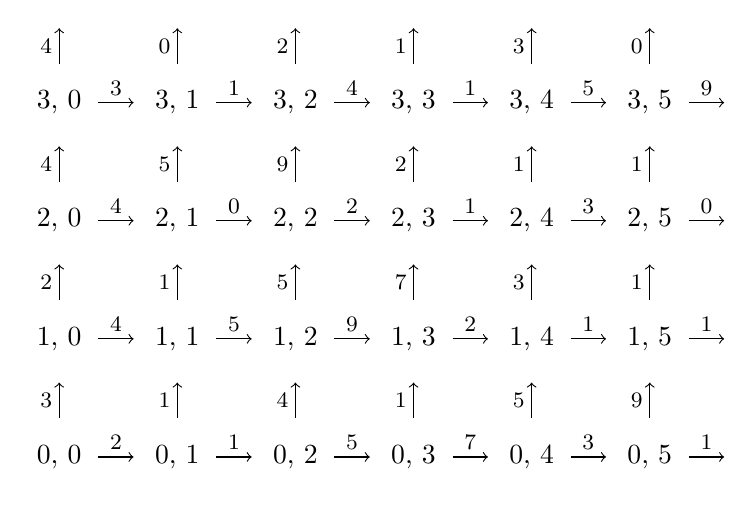
\begin{tikzpicture}[scale=1.5]
  \def\numberlist{{
      "0, 0","0, 1","0, 2","0, 3","0, 4","0, 5",
      "1, 0","1, 1","1, 2","1, 3","1, 4","1, 5",
      "2, 0","2, 1","2, 2","2, 3","2, 4","2, 5",
      "3, 0","3, 1","3, 2","3, 3","3, 4","3, 5"
    }}
  \def\edgelistA{{"3", "1", "4", "1", "5", "9", "2", "1", "5", "7", "3", "1", "4", "5", "9", "2", "1", "1", "4", "0", "2", "1", "3", "0"}}
  \def\edgelistB{{"2", "1", "5", "7", "3", "1", "4", "5", "9", "2", "1", "1", "4", "0", "2", "1", "3", "0", "3", "1", "4", "1", "5", "9"}}
  \def\maxX{5}
  \def\maxY{3}
  \foreach \x [count=\n] in {0,...,\maxX}{
    \foreach \y in {0,...,\maxY}{
      \pgfmathtruncatemacro\tmp{\n+(\maxX+1)*\y}
      \ifthenelse{\y=\maxY}{}{\draw[->] (\x,\y+0.33) -- (\x,\y+0.63)
        node [midway,left=-1pt,font=\footnotesize]
        {\pgfmathparse{\edgelistA[\tmp-1]}\pgfmathresult}; 
      }
      \ifthenelse{\x=\maxX}{}{\draw[->] (\x+0.33,\y) -- (\x+0.63,\y)
        node [midway,above=-1pt,font=\footnotesize]
        {\pgfmathparse{\edgelistB[\tmp-1]}\pgfmathresult};
      }
      % \node[shape=circle, draw=black, font=\small \sf] at (\x,\y) {\pgfmathparse{\numberlist[\tmp-1]}\pgfmathresult};
      \node[draw=none] at (\x, \y) {\NODEone{\pgfmathparse{\numberlist[\tmp-1]}\pgfmathresult}}; 
      }
    }
\end{tikzpicture}
\end{center}


\refreshHeader 
% \newpage

% \setlength{\ITEMHT}{0.4in}
% {\injectEnumerate
\inputAnswer{problem_1_answer}
% }

%%%%%%%%%%%%%%%%%%%%%%%%%%%%%%%%%%%%%%%%%%%%%%%%%%%%%%%%%%%% 
%%%%%%%%%%%%%%%%%%%%%%%%%%%%%%%%%%%%%%%%%%%%%%%%%%%%%%%%%%%% 
%%%%%%%%%%%%%%%%%%%%%%%%%%%%%%%%%%%%%%%%%%%%%%%%%%%%%%%%%%%% 
%%%%%%%%%%%%%%%%%%%%%%%%%%%%%%%%%%%%%%%%%%%%%%%%%%%%%%%%%%%% 

%%%%% EDIT THE FILES NAMED problem_X_answer.tex.  DON'T EDIT THIS FILE 

%%%%%%%%%%%%%%%% PROBLEM 2  %%%%%%%%%%%%%%%%%

\newpage

\problem \emph{(Section 7.3)}

Consider making change for total $T=10$ using denominations $D=\{1, 3, 4\}$.

\begin{enumerate}[label=(\alph*)]
  
\item Simulate the iterative \textsf{makeChange} algorithm in Section 7.3 on this input.
  What are the values in the array $m[0..T]$ computed by the algorithm?

% [review 2026-09-27] fix: D: stale section number 'Section 3.1' (old per-note numbering) -> 'Section 7.3.1' (Reducing to Shortest Path in a DAG)
\item Following Section 7.3.1, the corresponding DAG $G=(V, E)$ is shown below.
  What path in this DAG corresponds to making change with coins $4,3,1,1,1$ (in that order)?
  List the six nodes on the path.
\end{enumerate}

\begin{center}
  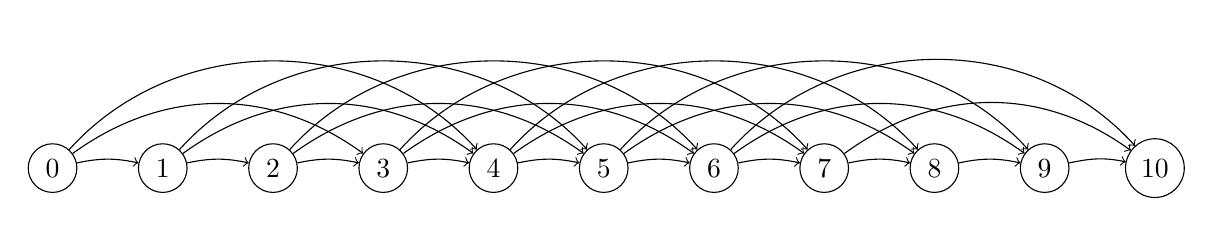
\begin{tikzpicture}[scale=1.4]
    \def\maxT{10}
    \foreach \x in {0,...,\maxT}{
      % \node[shape=circle, draw=black, font=\small \sf] at (\x,\y) {\pgfmathparse{\numberlist[\tmp-1]}\pgfmathresult};
      \node[draw=black,circle] (n\x) at (\x, 0) {\x}; 
    }
    \foreach \d in {1,3,4}{
      \foreach \x [count=\a from 0] in {\d,...,\maxT}{
        \draw[->] (n\a) to[out=12*\d,in=180-12*\d] (n\x);
      }
    }
  \end{tikzpicture}
\end{center}

\setlength{\ITEMHT}{1.5in}
{\injectEnumerate
  \inputAnswer{problem_2_answer}
}

%%%%%%%%%%%%%%%%%%%%%%%%%%%%%%%%%%%%%%%%%%%%%%%%%%%%%%%%%%%% 
%%%%%%%%%%%%%%%%%%%%%%%%%%%%%%%%%%%%%%%%%%%%%%%%%%%%%%%%%%%% 
%%%%%%%%%%%%%%%%%%%%%%%%%%%%%%%%%%%%%%%%%%%%%%%%%%%%%%%%%%%% 
%%%%%%%%%%%%%%%%%%%%%%%%%%%%%%%%%%%%%%%%%%%%%%%%%%%%%%%%%%%% 

%%%%% EDIT THE FILES NAMED problem_X_answer.tex.  DON'T EDIT THIS FILE 

%%%%%%%%%%%%%%%% PROBLEM 3  %%%%%%%%%%%%%%%%%

\newpage

\problem \emph{(Section 7.3)}
Consider the following problem, \prob{Counting Ways to Make Change}:

\begin{mylist}
\item[\bf input:]
  A pair $I=(D, T)$ where
  $D=\{d_1, d_2, \ldots, d_k\}$
  is a set of \emph{denominations},
  and $T$ is a target
  (all non-negative integers, with $1\in D$).

\item[\bf output:]
  The number of sequences $C=(c_1, \ldots, c_\ell)$
  s.t.~$c_i\in D$ for all $i$
  and $\sum_i c_i = T$.
\end{mylist}

For example, with $D=\{1, 3\}$ and $T=4$, there are three: $(1, 1, 1, 1)$, $(1, 3)$, and $(3, 1)$.

Adapt the algorithm for Making Change from Section 7.3 to solve this problem.
Use the first two steps from Section 7.4 to define your algorithm:

\begin{enumerate}[label=(\alph*)]

\item Define the subproblems.

\item State the recurrence relation.

\item Give pseudo-code for an iterative implementation of the algorithm.
  
\end{enumerate}

\continued

\setlength{\ITEMHT}{2in}
{\injectEnumerate
  \inputAnswer{problem_3_answer}
}

%%%%%%%%%%%%%%%%%%%%%%%%%%%%%%%%%%%%%%%%%%%%%%%%%%%%%%%%%%%% 
%%%%%%%%%%%%%%%%%%%%%%%%%%%%%%%%%%%%%%%%%%%%%%%%%%%%%%%%%%%% 
%%%%%%%%%%%%%%%%%%%%%%%%%%%%%%%%%%%%%%%%%%%%%%%%%%%%%%%%%%%% 
%%%%%%%%%%%%%%%%%%%%%%%%%%%%%%%%%%%%%%%%%%%%%%%%%%%%%%%%%%%% 

%%%%% EDIT THE FILES NAMED problem_X_answer.tex.  DON'T EDIT THIS FILE 

%%%%%%%%%%%%%%%% PROBLEM 4  %%%%%%%%%%%%%%%%%

\newpage
\problem \emph{(Exercise 5.10)}
Is the following conjecture true or false?
Either give a long-form proof of the conjecture (as a theorem),
or prove that it is false by giving a counter-example,
and explaining clearly how the algorithm fails on your counter-example.

\begin{conjecture}\label{dijkstra 2}
  Let $G=(V,E)$ be any edge-weighted digraph, and $s\in V$ any vertex.
  Suppose that every edge that doesn't touch $s$ has non-negative weight.
  (That is, for every edge $(u,w)\in E$, if $s\not\in \{u,w\}$, then $\weight {u,w} \ge 0$.
  Edges entering or leaving $s$ can have negative weight.)
  Suppose also that $G$ has no negative-weight cycles. 
  Then Dijkstra's algorithm, if run on input $(G,s)$,
  correctly computes the shortest-path distance from $s$ to each vertex $v\in V$.
\end{conjecture}

If you try to prove it, your proof should be \emph{as similar as possible}
to the proof of correctness for Dijkstra's algorithm in Section 5.8.
(Your score will depend on how similar your proof is.)
We'll provide that proof as a template.
Please color all text that you add to it \BLUE{blue}.
You may use Observation 5.7 (Section 5.8) without proof --- but if you do, cite it where you use it.

\bigskip

For reference, here is the algorithm:

\begin{samepage}
  \begin{myframed}
    \begin{steps}
    \item[$\textsf{Dijkstra}\big(G=(V,E), s\big)$:]
      \comment{\normalsize --- Dijkstra's algorithm for \prob{Single-Source Shortest Paths} ---} 
      \step initialize $K \leftarrow \{s\}$ and $d[s] = 0$
      \step[loop] while some edge in $E$ leaves $K$
      (that is, $\exists (u,w) \in E: u\in K,~w\not\in K$):
      \begin{block}
        \step among edges leaving $K$,
        choose edge $(u',w')$ that minimizes $d[u'] + \weight {u', w'}$
        \step set $d[w'] = d[u'] + \weight {u', w'}$
        \step add $w'$ to $K$
      \end{block}
      \step\label{unreachable}
      set $d[w] = \infty$ for all $w\in V\setminus K$
      \step return $d$
    \end{steps}
  \end{myframed}
\end{samepage}

Note that in the proof of Lemma 1, in Step 3.12.5, it can happen that $\weight {P_y} < 0$.
Consider the graph below, with $K=\{s,x,u\}$ and path $P=(s,x,y,s,w)$.
(And $d[s]=0$, $d[u] = d[x] = 1$.)

\begin{center}
  \begin{tikzpicture}[
      vertex/.style={circle, draw},
      every path/.style={->}
    ]
    \node[vertex] (s) {s}; 
    \node[vertex] (x) [below =of s, xshift=-15pt] {x}; 
    \node[vertex] (y) [below =of x, xshift=-30pt] {y}; 
    \node[vertex] (u) [below =of s, xshift=15pt] {u}; 
    \node[vertex] (w) [below =of u, xshift=30pt] {w};
    
    \draw (s) -- (x) node [midway, left] {1};
    \draw (x) -- (y) node [midway, left] {3};
    \draw (s) -- (u) node [midway, right] {1};
    \draw (u) -- (w) node [midway, right] {1}; 
    \draw (y) to [bend left=40] node [midway, left] {-4} (s); 
    \draw (s) to [bend left=40] node [midway, right] {3} (w); 

    \draw (0, -1) node[draw=black,dashed,circle,minimum size=3cm] {$K$};
  \end{tikzpicture}
\end{center}

\inputAnswer{problem_4_answer}

\end{document}

%%% Local Variables:
%%% mode: latex
%%% TeX-master: t
%%% End:
